\let\negmedspace\undefined
\let\negthickspace\undefined
\documentclass[journal,12pt,onecolumn]{IEEEtran}
\usepackage{cite}
\usepackage{amsmath,amssymb,amsfonts,amsthm}
\usepackage{algorithmic}
\usepackage{graphicx}
\graphicspath{{./figs/}}
\usepackage{textcomp}
\usepackage{xcolor}
\usepackage{txfonts}
\usepackage{listings}
\usepackage{enumitem}
\usepackage{mathtools}
\usepackage{gensymb}
\usepackage{comment}
\usepackage{caption}
\usepackage[breaklinks=true]{hyperref}
\usepackage{tkz-euclide} 
\usepackage{listings}
\usepackage{gvv}                                        
%\def\inputGnumericTable{}                                 
\usepackage[latin1]{inputenc}     
\usepackage{xparse}
\usepackage{color}                                            
\usepackage{array}                                            
\usepackage{longtable}                                       
\usepackage{calc}                                             
\usepackage{multirow}
\usepackage{multicol}
\usepackage{hhline}                                           
\usepackage{ifthen}                                           
\usepackage{lscape}
\usepackage{tabularx}
\usepackage{array}
\usepackage{float}

\begin{document}

\title{11.2.7}
\author{AI25BTECH11001 - ABHISEK MOHAPATRA}
{\let\newpage\relax\maketitle}
	
	 	\textbf{Question}:
	A line through the mid-point of a side of a triangle parallel to another side bisects
the third side.	

		\textbf{Solution:}

	Graph:
\begin{figure}[h!]
	\centering
	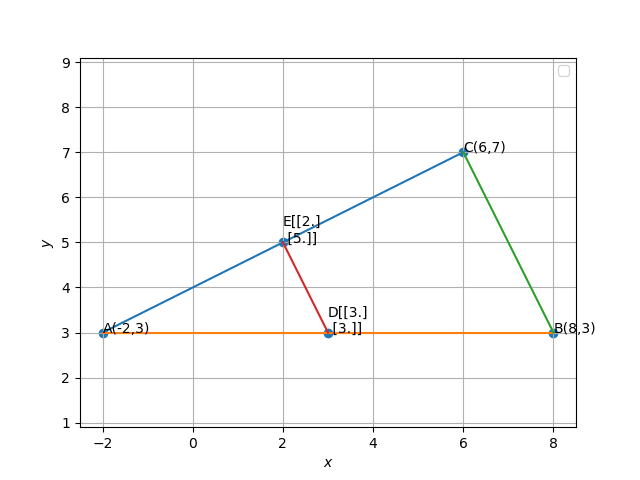
\includegraphics[width=0.55\linewidth]{img.png}
\end{figure}


Consider a triangle $\Delta \vec{ABC}$.
Let $\vec{D}$ and $\vec{E}$ are midpoints on the sides opposite to $\vec{C}$ and $\vec{B}$.
So,
\begin{align}
		\vec{D} = \frac{\vec{A} +\vec{B}}{2}, 
		\vec{E} = \frac{\vec{A} +\vec{C}}{2}
\end{align}
so the line joining the midpoints is
\begin{align}
		\vec{D} - \vec{E} =\frac{\vec{A} +\vec{B}}{2}-\frac{\vec{A} +\vec{C}}{2}
		=\frac{\vec{B} -\vec{C}}{2}
		=\frac{1}{2}\brak{\vec{B} -\vec{C}} = \lambda\brak{\vec{B} -\vec{C}}
\end{align}

So, the line is parallel to the third side as it $\lambda\brak{\vec{B} -\vec{C}}$.

Hence, proved.

\end{document}



